% ============================================================
% CHAPITRE 4 : ARCHITECTURE DU SYSTÈME
% ============================================================

\chapter{Architecture du Système}

\section{Introduction}

Ce chapitre présente l'architecture détaillée du système DMS, décomposée en modules fonctionnels interconnectés. L'accent est mis sur la communication entre les composants matériels (caméra, ECU, actionneurs) et les protocoles utilisés, conformément aux standards de l'industrie automobile.

\section{Vue d'Ensemble de l'Architecture}

Le système DMS est structuré en \textbf{6 modules fonctionnels} principaux, formant un pipeline de traitement temps réel :

\begin{figure}[H]
\centering
\begin{tikzpicture}[
    module/.style={rectangle, draw, thick, fill=#1, text width=3.2cm, text centered, minimum height=1.8cm, rounded corners=5pt, font=\small\bfseries},
    submodule/.style={rectangle, draw, fill=#1, text width=2.5cm, text centered, minimum height=0.8cm, rounded corners=2pt, font=\tiny},
    arrow/.style={->, >=stealth, very thick, color=stellantisblue},
    data/.style={->, >=stealth, thick, dashed, color=green!50!black},
    node distance=1.8cm
]
    % Modules principaux
    \node[module=blue!15] (acq) {1. Acquisition\\Vidéo};
    \node[module=orange!15, right=of acq] (detect) {2. Détection\\Visage/Yeux};
    \node[module=purple!15, right=of detect] (pose) {3. Estimation\\Pose Tête};
    \node[module=red!15, below=2cm of acq] (analyse) {4. Analyse\\Comportementale};
    \node[module=yellow!20, below=2cm of detect] (ecu) {5. Logique\\ECU};
    \node[module=green!20, below=2cm of pose] (alert) {6. Système\\d'Alertes};
    
    % Flèches principales
    \draw[arrow] (acq) -- node[above, font=\tiny] {images} (detect);
    \draw[arrow] (detect) -- node[above, font=\tiny] {landmarks} (pose);
    \draw[arrow] (detect) -- node[left, font=\tiny, text width=1.5cm, align=center] {état yeux\\confiance} (analyse);
    \draw[arrow] (pose) -- node[right, font=\tiny, text width=1.5cm, align=center] {yaw, pitch\\roll} (analyse);
    \draw[arrow] (analyse) -- node[above, font=\tiny] {scores} (ecu);
    \draw[arrow] (ecu) -- node[above, font=\tiny] {commandes} (alert);
    
    % Cadre global
    \node[draw, dashed, thick, fit=(acq)(detect)(pose)(analyse)(ecu)(alert), inner sep=0.7cm, label=above:{\large\textbf{Architecture Globale du Système DMS}}] {};
    
\end{tikzpicture}
\caption{Architecture modulaire globale du système DMS.}
\label{fig:archi_globale}
\end{figure}

\section{Module d'Acquisition Vidéo}

\subsection{Description Fonctionnelle}

Le module d'acquisition vidéo gère la capture d'images à partir d'une source vidéo (caméra USB, caméra IR, ou fichier vidéo). Il constitue la première étape du pipeline de traitement.

\subsection{Spécifications Techniques}

\begin{table}[H]
\centering
\caption{Spécifications du module d'acquisition vidéo.}
\label{tab:video_specs}
\renewcommand{\arraystretch}{1.3}
\begin{tabular}{|l|l|}
\hline
\rowcolor{stellantisblue!15}
\textbf{Paramètre} & \textbf{Valeur} \\
\hline
Résolution & $640 \times 480$ pixels (par défaut) \\
\hline
Fréquence d'images & 30 FPS (configurable : 15--60 FPS) \\
\hline
Format d'entrée & BGR (OpenCV), niveaux de gris pour CNN \\
\hline
Sources supportées & Caméra USB, fichier vidéo (.mp4, .avi), images synthétiques \\
\hline
Prétraitement & Conversion en niveaux de gris, égalisation d'histogramme \\
\hline
Interface de sortie & Générateur Python (yield image par image) \\
\hline
\end{tabular}
\end{table}

\subsection{Prétraitement de l'Image}

Le prétraitement de chaque image suit les étapes suivantes :

\begin{enumerate}[leftmargin=2cm]
    \item \textbf{Conversion couleur} : BGR $\rightarrow$ niveaux de gris ($Y = 0.299R + 0.587G + 0.114B$)
    \item \textbf{Égalisation d'histogramme} : Amélioration du contraste par redistribution uniforme des niveaux de gris :
\end{enumerate}

\begin{equation}
H(v) = \text{round}\left(\frac{\text{CDF}(v) - \text{CDF}_{\min}}{(M \times N) - \text{CDF}_{\min}} \times (L - 1)\right)
\label{eq:hist_equalization}
\end{equation}

où $\text{CDF}(v)$ est la fonction de distribution cumulative, $M \times N$ la taille de l'image et $L$ le nombre de niveaux de gris (256).

\section{Module de Détection Visage et Yeux}

\subsection{Pipeline de Détection}

Ce module combine deux approches complémentaires pour une détection robuste :

\begin{figure}[H]
\centering
\begin{tikzpicture}[
    block/.style={rectangle, draw, fill=#1, text width=2.8cm, text centered, minimum height=1cm, rounded corners=3pt, font=\small},
    decision/.style={diamond, draw, fill=yellow!20, text width=1.5cm, text centered, aspect=2, font=\tiny},
    arrow/.style={->, >=stealth, thick}
]
    \node[block=gray!15] (input) {Image\\niveaux de gris};
    \node[block=blue!15, right=1.5cm of input] (haar) {Cascade\\de Haar};
    \node[decision, right=1.5cm of haar] (faces) {Visage(s)\\détecté(s)?};
    \node[block=orange!15, right=1.5cm of faces] (cnn_face) {CNN\\Validation\\Visage};
    \node[block=purple!15, below=1.5cm of haar] (haar_eyes) {Cascade\\Haar Yeux};
    \node[block=red!15, below=1.5cm of cnn_face] (cnn_eyes) {CNN\\Classification\\Yeux};
    \node[block=green!15, below=1.5cm of $(haar_eyes)!0.5!(cnn_eyes)$] (output) {Résultat :\\état + confiance};
    
    \draw[arrow] (input) -- (haar);
    \draw[arrow] (haar) -- (faces);
    \draw[arrow] (faces) -- node[above, font=\tiny] {oui} (cnn_face);
    \draw[arrow] (cnn_face) -- (cnn_eyes);
    \draw[arrow] (faces) |- node[right, font=\tiny, pos=0.3] {oui} (haar_eyes);
    \draw[arrow] (haar_eyes) -- (cnn_eyes);
    \draw[arrow] (cnn_eyes) -- (output);
    
\end{tikzpicture}
\caption{Pipeline de détection visage et yeux.}
\label{fig:detection_pipeline}
\end{figure}

\subsection{Architecture du Face Detection CNN}

Le réseau \keyword{FaceDetectionCNN} valide les détections de la cascade de Haar et attribue un score de confiance :

\begin{table}[H]
\centering
\caption{Architecture détaillée du FaceDetectionCNN.}
\label{tab:face_cnn}
\renewcommand{\arraystretch}{1.3}
\begin{tabularx}{\textwidth}{|c|l|l|c|c|}
\hline
\rowcolor{stellantisblue!15}
\textbf{\#} & \textbf{Couche} & \textbf{Paramètres} & \textbf{Sortie} & \textbf{Nb Param.} \\
\hline
1 & Conv2D + BN + ReLU & 16 filtres, $3 \times 3$, padding=1 & $64 \times 64 \times 16$ & 176 \\
\hline
2 & MaxPool2D & $2 \times 2$, stride=2 & $32 \times 32 \times 16$ & 0 \\
\hline
3 & Conv2D + BN + ReLU & 32 filtres, $3 \times 3$, padding=1 & $32 \times 32 \times 32$ & 4\,672 \\
\hline
4 & MaxPool2D & $2 \times 2$, stride=2 & $16 \times 16 \times 32$ & 0 \\
\hline
5 & Conv2D + BN + ReLU & 64 filtres, $3 \times 3$, padding=1 & $16 \times 16 \times 64$ & 18\,560 \\
\hline
6 & MaxPool2D & $2 \times 2$, stride=2 & $8 \times 8 \times 64$ & 0 \\
\hline
7 & Conv2D + BN + ReLU & 128 filtres, $3 \times 3$, padding=1 & $8 \times 8 \times 128$ & 73\,984 \\
\hline
8 & AdaptiveAvgPool & $1 \times 1$ & 128 & 0 \\
\hline
9 & FC + ReLU + Dropout(0.5) & 64 neurones & 64 & 8\,256 \\
\hline
10 & FC (Sortie) & 2 classes & 2 & 130 \\
\hline
\multicolumn{4}{|r|}{\textbf{Total des paramètres}} & \textbf{105\,778} \\
\hline
\end{tabularx}
\end{table}

\subsection{Architecture du Eye State CNN}

Le réseau \keyword{EyeStateCNN} classifie l'état des yeux en deux catégories : ouvert ou fermé.

\begin{table}[H]
\centering
\caption{Architecture détaillée du EyeStateCNN.}
\label{tab:eye_cnn}
\renewcommand{\arraystretch}{1.3}
\begin{tabularx}{\textwidth}{|c|l|l|c|c|}
\hline
\rowcolor{stellantisblue!15}
\textbf{\#} & \textbf{Couche} & \textbf{Paramètres} & \textbf{Sortie} & \textbf{Nb Param.} \\
\hline
1 & Conv2D + BN + ReLU & 32 filtres, $3 \times 3$, padding=1 & $24 \times 24 \times 32$ & 352 \\
\hline
2 & MaxPool2D & $2 \times 2$, stride=2 & $12 \times 12 \times 32$ & 0 \\
\hline
3 & Conv2D + BN + ReLU & 64 filtres, $3 \times 3$, padding=1 & $12 \times 12 \times 64$ & 18\,560 \\
\hline
4 & MaxPool2D & $2 \times 2$, stride=2 & $6 \times 6 \times 64$ & 0 \\
\hline
5 & Conv2D + BN + ReLU & 128 filtres, $3 \times 3$, padding=1 & $6 \times 6 \times 128$ & 73\,984 \\
\hline
6 & MaxPool2D & $2 \times 2$, stride=2 & $3 \times 3 \times 128$ & 0 \\
\hline
7 & FC + ReLU + Dropout(0.5) & 256 neurones & 256 & 295\,168 \\
\hline
8 & FC (Sortie) & 2 classes & 2 & 514 \\
\hline
\multicolumn{4}{|r|}{\textbf{Total des paramètres}} & \textbf{388\,578} \\
\hline
\end{tabularx}
\end{table}

Le flux de calcul à travers le réseau peut être formalisé comme suit :

\begin{align}
\mathbf{h}_1 &= \text{MaxPool}\left(\text{ReLU}\left(\text{BN}\left(\text{Conv}_{32}^{3\times3}(\mathbf{x})\right)\right)\right) \in \mathbb{R}^{12 \times 12 \times 32} \label{eq:layer1} \\
\mathbf{h}_2 &= \text{MaxPool}\left(\text{ReLU}\left(\text{BN}\left(\text{Conv}_{64}^{3\times3}(\mathbf{h}_1)\right)\right)\right) \in \mathbb{R}^{6 \times 6 \times 64} \label{eq:layer2} \\
\mathbf{h}_3 &= \text{MaxPool}\left(\text{ReLU}\left(\text{BN}\left(\text{Conv}_{128}^{3\times3}(\mathbf{h}_2)\right)\right)\right) \in \mathbb{R}^{3 \times 3 \times 128} \label{eq:layer3} \\
\mathbf{f} &= \text{flatten}(\mathbf{h}_3) \in \mathbb{R}^{1152} \label{eq:flatten} \\
\mathbf{h}_4 &= \text{Dropout}_{0.5}\left(\text{ReLU}\left(\mathbf{W}_1 \mathbf{f} + \mathbf{b}_1\right)\right) \in \mathbb{R}^{256} \label{eq:fc1} \\
\mathbf{y} &= \mathbf{W}_2 \mathbf{h}_4 + \mathbf{b}_2 \in \mathbb{R}^{2} \label{eq:fc2}
\end{align}

La prédiction finale est obtenue par la fonction softmax :

\begin{equation}
P(\text{classe}_k | \mathbf{x}) = \frac{e^{y_k}}{\sum_{j=1}^{2} e^{y_j}}, \quad k \in \{\text{ouvert}, \text{fermé}\}
\label{eq:softmax}
\end{equation}

\section{Module d'Estimation de la Pose de la Tête}

\subsection{Principe de Fonctionnement}

L'estimation de la pose utilise 6 points de repère faciaux (\textit{landmarks}) clés et un modèle 3D générique du visage pour résoudre le problème PnP via la fonction \texttt{cv2.solvePnP} d'OpenCV.

\begin{figure}[H]
\centering
\begin{tikzpicture}[
    block/.style={rectangle, draw, fill=#1, text width=3cm, text centered, minimum height=1.2cm, rounded corners=3pt, font=\small},
    arrow/.style={->, >=stealth, thick}
]
    \node[block=blue!15] (landmarks) {6 Points 2D\\(landmarks)};
    \node[block=orange!15, below=1cm of landmarks] (model3d) {Modèle 3D\\du visage};
    \node[block=purple!15, right=2.5cm of $(landmarks)!0.5!(model3d)$] (pnp) {solvePnP\\(OpenCV)};
    \node[block=green!15, right=2.5cm of pnp] (angles) {Angles d'Euler\\(Yaw, Pitch, Roll)};
    
    \draw[arrow] (landmarks) -| (pnp);
    \draw[arrow] (model3d) -| (pnp);
    \draw[arrow] (pnp) -- (angles);
    
\end{tikzpicture}
\caption{Pipeline d'estimation de la pose de la tête.}
\label{fig:head_pose_pipeline}
\end{figure}

\subsection{Points de Repère 3D du Visage}

Le modèle 3D générique utilise les coordonnées suivantes (en millimètres) :

\begin{table}[H]
\centering
\caption{Coordonnées 3D des points de repère du visage.}
\label{tab:3d_landmarks}
\renewcommand{\arraystretch}{1.3}
\begin{tabular}{|l|c|c|c|}
\hline
\rowcolor{stellantisblue!15}
\textbf{Point} & \textbf{X (mm)} & \textbf{Y (mm)} & \textbf{Z (mm)} \\
\hline
Bout du nez & 0.0 & 0.0 & 0.0 \\
\hline
Menton & 0.0 & $-330.0$ & $-65.0$ \\
\hline
Coin gauche de l'œil gauche & $-225.0$ & 170.0 & $-135.0$ \\
\hline
Coin droit de l'œil droit & 225.0 & 170.0 & $-135.0$ \\
\hline
Coin gauche de la bouche & $-150.0$ & $-150.0$ & $-125.0$ \\
\hline
Coin droit de la bouche & 150.0 & $-150.0$ & $-125.0$ \\
\hline
\end{tabular}
\end{table}

\subsection{Résolution du Problème PnP}

L'algorithme \texttt{solvePnP} d'OpenCV résout le système suivant pour trouver le vecteur de rotation $\mathbf{r}$ (Rodrigues) et le vecteur de translation $\mathbf{t}$ :

\begin{equation}
\min_{\mathbf{r}, \mathbf{t}} \sum_{i=1}^{6} \left\| \mathbf{p}_i^{2D} - \pi(\mathbf{K}, \mathbf{r}, \mathbf{t}, \mathbf{P}_i^{3D}) \right\|^2
\label{eq:pnp_optimization}
\end{equation}

où $\pi$ est la fonction de projection perspective et $\mathbf{p}_i^{2D}$, $\mathbf{P}_i^{3D}$ sont les correspondances 2D-3D.

La conversion du vecteur de Rodrigues en matrice de rotation utilise la formule :

\begin{equation}
\mathbf{R} = \cos\theta \cdot \mathbf{I} + (1 - \cos\theta) \cdot \hat{\mathbf{r}} \hat{\mathbf{r}}^T + \sin\theta \cdot [\hat{\mathbf{r}}]_\times
\label{eq:rodrigues}
\end{equation}

où $\theta = \|\mathbf{r}\|$, $\hat{\mathbf{r}} = \mathbf{r}/\theta$, et $[\hat{\mathbf{r}}]_\times$ est la matrice antisymétrique.

\section{Module d'Analyse Comportementale}

\subsection{Architecture du Module}

Ce module maintient un historique glissant des observations sur une fenêtre temporelle configurable (par défaut $W = 60$ secondes) et calcule les indicateurs en continu.

\subsection{Calcul Détaillé du PERCLOS}

Le PERCLOS est mis à jour à chaque nouvelle image en utilisant un tampon circulaire (\textit{deque}) :

\begin{equation}
\text{PERCLOS}(t) = \frac{\sum_{i=t-W}^{t} \mathbb{1}[\text{état}_i = \text{fermé}]}{|W|} \times 100\%
\label{eq:perclos_detailed}
\end{equation}

où $\mathbb{1}[\cdot]$ est la fonction indicatrice et $|W|$ le nombre d'images dans la fenêtre.

\subsection{Calcul du Score de Fatigue}

Le score de fatigue combine quatre composantes pondérées :

\begin{equation}
\boxed{
S_{\text{fatigue}} = w_1 \cdot C_{\text{PERCLOS}} + w_2 \cdot C_{\text{blink}} + w_3 \cdot C_{\text{duration}} + w_4 \cdot C_{\text{closure}}
}
\label{eq:fatigue_score}
\end{equation}

avec les poids $w_1 = 0.4$, $w_2 = 0.2$, $w_3 = 0.2$, $w_4 = 0.2$, et :

\begin{align}
C_{\text{PERCLOS}} &= \min\left(\frac{\text{PERCLOS}}{100}, 1.0\right) \label{eq:c_perclos} \\
C_{\text{blink}} &= \begin{cases}
    \frac{|f_{\text{blink}} - f_{\text{normal}}|}{f_{\text{normal}}} & \text{si anormal} \\
    0 & \text{si } 10 \leq f_{\text{blink}} \leq 20
\end{cases} \label{eq:c_blink} \\
C_{\text{duration}} &= \min\left(\frac{\bar{d}_{\text{blink}}}{\tau_{\text{max}}}, 1.0\right) \label{eq:c_duration} \\
C_{\text{closure}} &= \min\left(\frac{d_{\text{current}}}{\tau_{\text{critical}}}, 1.0\right) \label{eq:c_closure}
\end{align}

où $f_{\text{normal}} = 17.5$ clig./min, $\tau_{\text{max}} = 0.5$ s, et $\tau_{\text{critical}} = 2.0$ s.

\subsection{Calcul du Score de Distraction}

Le score de distraction est calculé à partir de la pose de la tête :

\begin{equation}
\boxed{
S_{\text{distraction}} = 0.4 \cdot C_{\text{yaw}} + 0.2 \cdot C_{\text{pitch}} + 0.4 \cdot C_{\text{away}}
}
\label{eq:distraction_score}
\end{equation}

avec :

\begin{align}
C_{\text{yaw}} &= \min\left(\frac{|\text{yaw}|}{\theta_{\text{yaw,max}}}, 1.0\right), \quad \theta_{\text{yaw,max}} = 45° \label{eq:c_yaw} \\
C_{\text{pitch}} &= \min\left(\frac{|\text{pitch}|}{\theta_{\text{pitch,max}}}, 1.0\right), \quad \theta_{\text{pitch,max}} = 35° \label{eq:c_pitch} \\
C_{\text{away}} &= \begin{cases}
    1.0 & \text{si regard détourné} > 3\text{s} \\
    \frac{t_{\text{away}}}{3.0} & \text{sinon}
\end{cases} \label{eq:c_away}
\end{align}

\section{Module de Logique ECU}

\subsection{Machine à États}

La logique de décision est modélisée comme une machine à états finis avec 4 niveaux d'alerte :

\begin{figure}[H]
\centering
\begin{tikzpicture}[
    state/.style={circle, draw, thick, fill=#1, minimum size=2cm, text centered, font=\small\bfseries, text width=1.8cm},
    arrow/.style={->, >=stealth, thick},
    trans/.style={font=\tiny, text width=2cm, align=center}
]
    \node[state=green!30] (normal) at (0, 0) {NORMAL\\(0)};
    \node[state=alertyellow!40] (warning) at (5, 0) {WARNING\\(2)};
    \node[state=alertorange!40] (critical) at (10, 0) {CRITICAL\\(3)};
    \node[state=alertred!40] (emergency) at (10, -4) {EMERGENCY\\(4)};
    
    % Transitions
    \draw[arrow] (normal) -- node[above, trans] {$S_f > 0.35$\\ou\\$S_d > 0.35$} (warning);
    \draw[arrow] (warning) -- node[above, trans] {$S_f > 0.6$\\ou\\$S_d > 0.6$} (critical);
    \draw[arrow] (critical) -- node[right, trans] {$S_f > 0.75$} (emergency);
    
    % Retour
    \draw[arrow, bend right=30] (warning) to node[below, trans] {$S_f < 0.2$\\et $S_d < 0.2$} (normal);
    \draw[arrow, bend right=30] (critical) to node[below, trans] {$S_f < 0.5$} (warning);
    
    % Auto-transitions
    \draw[arrow] (normal) to[loop above] node[above, font=\tiny] {$S < 0.35$} (normal);
    
\end{tikzpicture}
\caption{Machine à états de la logique ECU du DMS.}
\label{fig:ecu_state_machine}
\end{figure}

\subsection{Niveaux d'Alerte et Actions}

\begin{table}[H]
\centering
\caption{Niveaux d'alerte du système ECU et actions associées.}
\label{tab:alert_levels}
\renewcommand{\arraystretch}{1.4}
\begin{tabularx}{\textwidth}{|c|l|c|X|}
\hline
\rowcolor{stellantisblue!15}
\textbf{Niveau} & \textbf{Nom} & \textbf{Code} & \textbf{Action} \\
\hline
\cellcolor{green!20} 0 & NONE & 0 & Fonctionnement normal, pas d'alerte \\
\hline
\cellcolor{alertyellow!30} 1 & WARNING & 2 & Alerte visuelle (LED orange), notification sur tableau de bord \\
\hline
\cellcolor{alertorange!30} 2 & CRITICAL & 3 & Alerte sonore (buzzer), vibration du volant, message d'urgence \\
\hline
\cellcolor{alertred!30} 3 & EMERGENCY & 4 & Freinage d'urgence assisté, activation des feux de détresse, appel d'urgence \\
\hline
\end{tabularx}
\end{table}

\subsection{Logique de Transition}

Les conditions de transition entre les états sont formalisées dans le tableau~\ref{tab:transitions} :

\begin{table}[H]
\centering
\caption{Conditions de transition de la machine à états ECU.}
\label{tab:transitions}
\renewcommand{\arraystretch}{1.3}
\begin{tabularx}{\textwidth}{|l|l|X|}
\hline
\rowcolor{stellantisblue!15}
\textbf{De} & \textbf{Vers} & \textbf{Condition} \\
\hline
NORMAL & WARNING & $S_f > 0.35$ ou $S_d > 0.35$ \\
\hline
WARNING & CRITICAL & $S_f > 0.6$ ou $S_d > 0.6$ \\
\hline
CRITICAL & EMERGENCY & $S_f > 0.75$ \\
\hline
WARNING & NORMAL & $S_f < 0.2$ et $S_d < 0.2$ (pendant $> 5$s) \\
\hline
CRITICAL & WARNING & $S_f < 0.5$ (pendant $> 3$s) \\
\hline
EMERGENCY & CRITICAL & $S_f < 0.6$ (après action du conducteur) \\
\hline
\end{tabularx}
\end{table}

\section{Communication entre Composants}

\subsection{Architecture de Communication Globale}

La communication entre les différents composants matériels du système suit une architecture hiérarchique :

\begin{figure}[H]
\centering
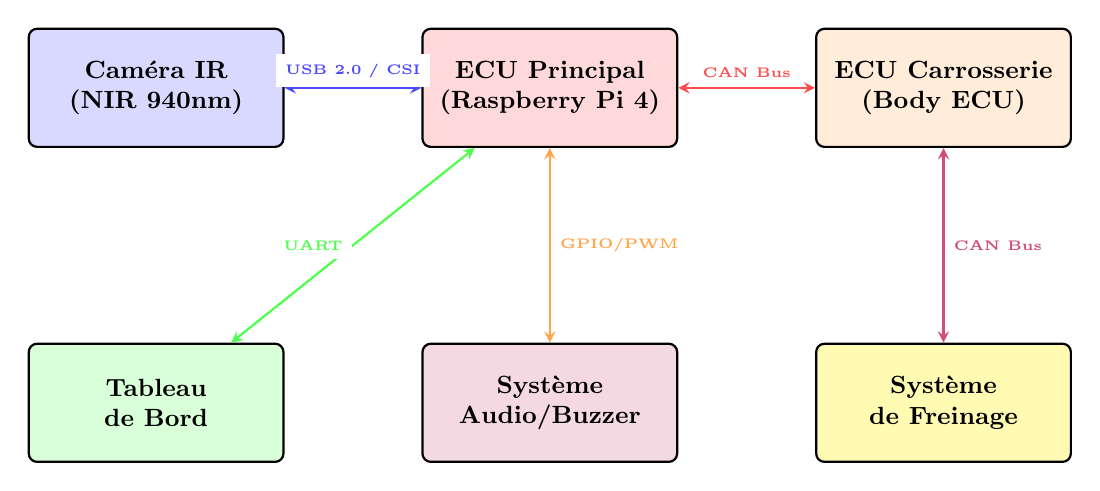
\begin{tikzpicture}[
    hw/.style={rectangle, draw, thick, fill=#1, text width=3cm, text centered, minimum height=1.5cm, rounded corners=3pt, font=\small\bfseries},
    bus/.style={rectangle, draw, thick, fill=gray!20, text width=2cm, text centered, minimum height=0.6cm, font=\tiny\bfseries},
    conn/.style={<->, >=stealth, thick, color=#1}
]
    % Composants matériels
    \node[hw=blue!15] (camera) at (0, 4) {Caméra IR\\(NIR 940nm)};
    \node[hw=red!15] (ecu_main) at (5, 4) {ECU Principal\\(Raspberry Pi 4)};
    \node[hw=orange!15] (ecu_body) at (10, 4) {ECU Carrosserie\\(Body ECU)};
    \node[hw=green!15] (display) at (0, 0) {Tableau\\de Bord};
    \node[hw=purple!15] (buzzer) at (5, 0) {Système\\Audio/Buzzer};
    \node[hw=yellow!30] (brake) at (10, 0) {Système\\de Freinage};
    
    % Bus de communication
    \draw[conn=blue!70] (camera) -- node[above, font=\tiny\bfseries, fill=white] {USB 2.0 / CSI} (ecu_main);
    \draw[conn=red!70] (ecu_main) -- node[above, font=\tiny\bfseries, fill=white] {CAN Bus} (ecu_body);
    \draw[conn=green!70] (ecu_main) -- node[left, font=\tiny\bfseries, fill=white] {UART} (display);
    \draw[conn=orange!70] (ecu_main) -- node[right, font=\tiny\bfseries, fill=white] {GPIO/PWM} (buzzer);
    \draw[conn=purple!70] (ecu_body) -- node[right, font=\tiny\bfseries, fill=white] {CAN Bus} (brake);
    
\end{tikzpicture}
\caption{Architecture de communication entre les composants matériels.}
\label{fig:communication_arch}
\end{figure}

\subsection{Communication Caméra $\rightarrow$ ECU}

\subsubsection{Interface Physique}

La caméra communique avec l'ECU principal via :
\begin{itemize}
    \item \textbf{USB 2.0} : Pour les caméras USB standard (débit : 480 Mbit/s)
    \item \textbf{CSI (\textit{Camera Serial Interface})} : Pour les caméras Raspberry Pi (débit : jusqu'à 1 Gbit/s)
\end{itemize}

\subsubsection{Protocole de Communication}

Le flux de données de la caméra vers l'ECU suit le protocole suivant :

\begin{enumerate}[leftmargin=2cm]
    \item \textbf{Acquisition} : La caméra capture une image au format RAW/YUYV
    \item \textbf{Transfert} : L'image est transférée via le bus USB/CSI vers le buffer mémoire
    \item \textbf{Décodage} : Le pilote vidéo (V4L2 sous Linux) décode l'image
    \item \textbf{Traitement} : OpenCV accède à l'image via l'API \texttt{cv2.VideoCapture}
\end{enumerate}

La latence de transfert est donnée par :

\begin{equation}
T_{\text{transfer}} = \frac{W \times H \times B_{\text{pp}}}{\text{Débit}_{\text{bus}}} \quad \text{(secondes)}
\label{eq:transfer_latency}
\end{equation}

Pour une image $640 \times 480$ en 8 bits/pixel via USB 2.0 :
\begin{equation}
T_{\text{transfer}} = \frac{640 \times 480 \times 8}{480 \times 10^6} \approx 5.12 \text{ ms}
\end{equation}

\subsection{Communication ECU $\rightarrow$ Actionneurs via CAN}

\subsubsection{Définition des Trames CAN DMS}

Les messages CAN envoyés par l'ECU DMS sont définis dans le tableau~\ref{tab:can_messages} :

\begin{table}[H]
\centering
\caption{Définition des trames CAN du système DMS.}
\label{tab:can_messages}
\renewcommand{\arraystretch}{1.3}
\begin{tabularx}{\textwidth}{|c|l|c|X|}
\hline
\rowcolor{stellantisblue!15}
\textbf{ID CAN} & \textbf{Nom} & \textbf{DLC} & \textbf{Contenu} \\
\hline
0x300 & DMS\_STATUS & 8 & Octet 0: Niveau d'alerte (0-4)\\& & & & Octets 1-2: Score fatigue ($\times 100$)\\& & & & Octets 3-4: Score distraction ($\times 100$)\\& & & & Octet 5: État conducteur (0-3)\\& & & & Octets 6-7: PERCLOS ($\times 100$) \\
\hline
0x301 & DMS\_ALERT & 4 & Octet 0: Type d'alerte\\& & & & Octet 1: Priorité\\& & & & Octets 2-3: Durée (ms) \\
\hline
0x302 & DMS\_HEAD\_POSE & 6 & Octets 0-1: Yaw ($\times 100$)\\& & & & Octets 2-3: Pitch ($\times 100$)\\& & & & Octets 4-5: Roll ($\times 100$) \\
\hline
0x303 & DMS\_EYE\_STATE & 4 & Octet 0: État yeux (0=ouvert, 1=fermé)\\& & & & Octet 1: Confiance ($\times 100$)\\& & & & Octets 2-3: EAR ($\times 1000$) \\
\hline
\end{tabularx}
\end{table}

\subsubsection{Format d'Encodage des Données}

Les données sont encodées en \textit{big-endian} avec les facteurs de mise à l'échelle suivants :

\begin{align}
\text{Score\_CAN} &= \text{round}(S_{\text{fatigue}} \times 100) \quad \text{(0 à 100)} \label{eq:can_score} \\
\text{Angle\_CAN} &= \text{round}(\theta \times 100) + 18000 \quad \text{(offset pour valeurs négatives)} \label{eq:can_angle}
\end{align}

\subsection{Communication ECU $\rightarrow$ Tableau de Bord via UART}

Pour le prototype, la communication avec le tableau de bord (écran LCD) utilise l'UART :

\begin{table}[H]
\centering
\caption{Configuration UART pour la communication avec le tableau de bord.}
\label{tab:uart_config}
\renewcommand{\arraystretch}{1.3}
\begin{tabular}{|l|l|}
\hline
\rowcolor{stellantisblue!15}
\textbf{Paramètre} & \textbf{Valeur} \\
\hline
Baudrate & 115\,200 bps \\
\hline
Bits de données & 8 \\
\hline
Parité & Aucune \\
\hline
Bits d'arrêt & 1 \\
\hline
Contrôle de flux & Aucun \\
\hline
\end{tabular}
\end{table}

Le format de la trame UART DMS est :

\begin{equation}
\text{Trame} = [\underbrace{0xAA}_{\text{Start}}][\underbrace{\text{CMD}}_{\text{1 octet}}][\underbrace{\text{LEN}}_{\text{1 octet}}][\underbrace{\text{DATA}}_{\text{N octets}}][\underbrace{\text{CRC}}_{\text{1 octet}}][\underbrace{0x55}_{\text{End}}]
\label{eq:uart_frame}
\end{equation}

\section{Diagramme de Séquence}

Le diagramme de séquence suivant illustre le flux de données complet lors d'une détection de fatigue :

\begin{figure}[H]
\centering
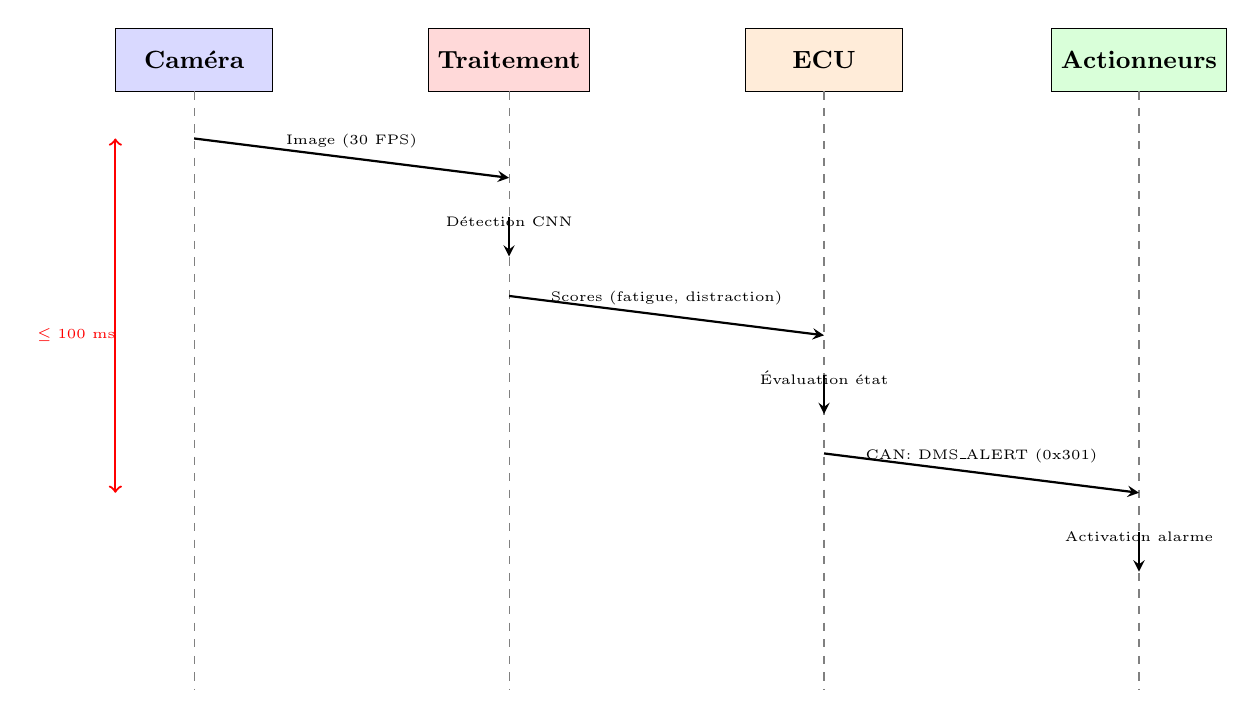
\begin{tikzpicture}[
    actor/.style={rectangle, draw, fill=#1, minimum width=2cm, minimum height=0.8cm, text centered, font=\small\bfseries},
    arrow/.style={->, >=stealth, thick},
    note/.style={font=\tiny, text width=3cm, align=center}
]
    % Acteurs
    \node[actor=blue!15] (cam) at (0, 0) {Caméra};
    \node[actor=red!15] (proc) at (4, 0) {Traitement};
    \node[actor=orange!15] (ecu) at (8, 0) {ECU};
    \node[actor=green!15] (act) at (12, 0) {Actionneurs};
    
    % Lignes de vie
    \foreach \x in {0, 4, 8, 12} {
        \draw[dashed, gray] (\x, -0.4) -- (\x, -8);
    }
    
    % Messages
    \draw[arrow] (0, -1) -- node[above, font=\tiny] {Image (30 FPS)} (4, -1.5);
    \draw[arrow] (4, -2) -- node[above, font=\tiny] {Détection CNN} (4, -2.5);
    \draw[arrow] (4, -3) -- node[above, font=\tiny] {Scores (fatigue, distraction)} (8, -3.5);
    \draw[arrow] (8, -4) -- node[above, font=\tiny] {Évaluation état} (8, -4.5);
    \draw[arrow] (8, -5) -- node[above, font=\tiny] {CAN: DMS\_ALERT (0x301)} (12, -5.5);
    \draw[arrow] (12, -6) -- node[above, font=\tiny] {Activation alarme} (12, -6.5);
    
    % Temps
    \node[font=\tiny, color=red] at (-1.5, -3.5) {$\leq 100$ ms};
    \draw[<->, red, thick] (-1, -1) -- (-1, -5.5);
    
\end{tikzpicture}
\caption{Diagramme de séquence pour une détection de fatigue.}
\label{fig:sequence_diagram}
\end{figure}

\section{Exigences de Performance}

\begin{table}[H]
\centering
\caption{Exigences de performance du système DMS.}
\label{tab:performance_requirements}
\renewcommand{\arraystretch}{1.3}
\begin{tabularx}{\textwidth}{|l|c|X|}
\hline
\rowcolor{stellantisblue!15}
\textbf{Exigence} & \textbf{Valeur Cible} & \textbf{Justification} \\
\hline
Latence bout-en-bout & $\leq 100$ ms & Temps de réaction acceptable pour la sécurité \\
\hline
Fréquence de traitement & $\geq 15$ FPS & Suivi fluide des clignements (durée min 100 ms) \\
\hline
Précision détection visage & $\geq 95\%$ & Fiabilité dans des conditions variées \\
\hline
Précision classification yeux & $\geq 90\%$ & Calcul précis du PERCLOS \\
\hline
Taux de faux positifs & $\leq 5\%$ & Éviter les alertes non justifiées \\
\hline
Consommation mémoire & $\leq 512$ Mo & Compatibilité avec ECU embarqué \\
\hline
\end{tabularx}
\end{table}

\section{Synthèse}

L'architecture proposée offre une conception modulaire et extensible, avec :
\begin{itemize}
    \item Une séparation claire des responsabilités entre les modules
    \item Des interfaces bien définies entre chaque composant
    \item Une communication standardisée via CAN et UART
    \item Des exigences de performance quantifiées et vérifiables
    \item Une logique ECU formalisée par une machine à états
\end{itemize}
